% REV00 Tue 04 May 2021 13:54:33 WIB
% START Tue 04 May 2021 13:54:33 WIB

\chapter{MR WEGG LOOKS AFTER HIMSELF}

Silas Wegg, being on his road to the Roman Empire, approaches it by way
of Clerkenwell. The time is early in the evening; the weather moist and
raw. Mr Wegg finds leisure to make a little circuit, by reason that he
folds his screen early, now that he combines another source of income
with it, and also that he feels it due to himself to be anxiously
expected at the Bower. ‘Boffin will get all the eagerer for waiting a
bit,’ says Silas, screwing up, as he stumps along, first his right eye,
and then his left. Which is something superfluous in him, for Nature has
already screwed both pretty tight.

‘If I get on with him as I expect to get on,’ Silas pursues, stumping
and meditating, ‘it wouldn’t become me to leave it here. It wouldn’t be
respectable.’ Animated by this reflection, he stumps faster, and looks
a long way before him, as a man with an ambitious project in abeyance
often will do.

Aware of a working-jeweller population taking sanctuary about the church
in Clerkenwell, Mr Wegg is conscious of an interest in, and a respect
for, the neighbourhood. But, his sensations in this regard halt as to
their strict morality, as he halts in his gait; for, they suggest the
delights of a coat of invisibility in which to walk off safely with the
precious stones and watch-cases, but stop short of any compunction for
the people who would lose the same.

Not, however, towards the ‘shops’ where cunning artificers work in
pearls and diamonds and gold and silver, making their hands so rich,
that the enriched water in which they wash them is bought for the
refiners;--not towards these does Mr Wegg stump, but towards the poorer
shops of small retail traders in commodities to eat and drink and keep
folks warm, and of Italian frame-makers, and of barbers, and of brokers,
and of dealers in dogs and singing-birds. From these, in a narrow and
a dirty street devoted to such callings, Mr Wegg selects one dark
shop-window with a tallow candle dimly burning in it, surrounded by a
muddle of objects vaguely resembling pieces of leather and dry stick,
but among which nothing is resolvable into anything distinct, save
the candle itself in its old tin candlestick, and two preserved frogs
fighting a small-sword duel. Stumping with fresh vigour, he goes in at
the dark greasy entry, pushes a little greasy dark reluctant side-door,
and follows the door into the little dark greasy shop. It is so dark
that nothing can be made out in it, over a little counter, but another
tallow candle in another old tin candlestick, close to the face of a man
stooping low in a chair.

Mr Wegg nods to the face, ‘Good evening.’

The face looking up is a sallow face with weak eyes, surmounted by a
tangle of reddish-dusty hair. The owner of the face has no cravat on,
and has opened his tumbled shirt-collar to work with the more ease.
For the same reason he has no coat on: only a loose waistcoat over his
yellow linen. His eyes are like the over-tried eyes of an engraver, but
he is not that; his expression and stoop are like those of a shoemaker,
but he is not that.

‘Good evening, Mr Venus. Don’t you remember?’

With slowly dawning remembrance, Mr Venus rises, and holds his candle
over the little counter, and holds it down towards the legs, natural and
artificial, of Mr Wegg.

‘To be SURE!’ he says, then. ‘How do you do?’

‘Wegg, you know,’ that gentleman explains.

‘Yes, yes,’ says the other. ‘Hospital amputation?’

‘Just so,’ says Mr Wegg.

‘Yes, yes,’ quoth Venus. ‘How do you do? Sit down by the fire, and warm
your--your other one.’

The little counter being so short a counter that it leaves the
fireplace, which would have been behind it if it had been longer,
accessible, Mr Wegg sits down on a box in front of the fire, and inhales
a warm and comfortable smell which is not the smell of the shop. ‘For
that,’ Mr Wegg inwardly decides, as he takes a corrective sniff or two,
‘is musty, leathery, feathery, cellary, gluey, gummy, and,’ with another
sniff, ‘as it might be, strong of old pairs of bellows.’

‘My tea is drawing, and my muffin is on the hob, Mr Wegg; will you
partake?’

It being one of Mr Wegg’s guiding rules in life always to partake, he
says he will. But, the little shop is so excessively dark, is stuck so
full of black shelves and brackets and nooks and corners, that he sees
Mr Venus’s cup and saucer only because it is close under the candle, and
does not see from what mysterious recess Mr Venus produces another
for himself until it is under his nose. Concurrently, Wegg perceives a
pretty little dead bird lying on the counter, with its head drooping
on one side against the rim of Mr Venus’s saucer, and a long stiff wire
piercing its breast. As if it were Cock Robin, the hero of the ballad,
and Mr Venus were the sparrow with his bow and arrow, and Mr Wegg were
the fly with his little eye.

Mr Venus dives, and produces another muffin, yet untoasted; taking the
arrow out of the breast of Cock Robin, he proceeds to toast it on the
end of that cruel instrument. When it is brown, he dives again and
produces butter, with which he completes his work.

Mr Wegg, as an artful man who is sure of his supper by-and-bye, presses
muffin on his host to soothe him into a compliant state of mind, or, as
one might say, to grease his works. As the muffins disappear, little by
little, the black shelves and nooks and corners begin to appear, and Mr
Wegg gradually acquires an imperfect notion that over against him on the
chimney-piece is a Hindoo baby in a bottle, curved up with his big
head tucked under him, as he would instantly throw a summersault if the
bottle were large enough.

When he deems Mr Venus’s wheels sufficiently lubricated, Mr Wegg
approaches his object by asking, as he lightly taps his hands together,
to express an undesigning frame of mind:

‘And how have I been going on, this long time, Mr Venus?’

‘Very bad,’ says Mr Venus, uncompromisingly.

‘What? Am I still at home?’ asks Wegg, with an air of surprise.

‘Always at home.’

This would seem to be secretly agreeable to Wegg, but he veils his
feelings, and observes, ‘Strange. To what do you attribute it?’

‘I don’t know,’ replies Venus, who is a haggard melancholy man, speaking
in a weak voice of querulous complaint, ‘to what to attribute it, Mr
Wegg. I can’t work you into a miscellaneous one, no how. Do what I will,
you can’t be got to fit. Anybody with a passable knowledge would pick
you out at a look, and say,--“No go! Don’t match!”’

‘Well, but hang it, Mr Venus,’ Wegg expostulates with some little
irritation, ‘that can’t be personal and peculiar in ME. It must often
happen with miscellaneous ones.’

‘With ribs (I grant you) always. But not else. When I prepare a
miscellaneous one, I know beforehand that I can’t keep to nature, and
be miscellaneous with ribs, because every man has his own ribs, and no
other man’s will go with them; but elseways I can be miscellaneous. I
have just sent home a Beauty--a perfect Beauty--to a school of art. One
leg Belgian, one leg English, and the pickings of eight other people in
it. Talk of not being qualified to be miscellaneous! By rights you OUGHT
to be, Mr Wegg.’

Silas looks as hard at his one leg as he can in the dim light, and after
a pause sulkily opines ‘that it must be the fault of the other people.
Or how do you mean to say it comes about?’ he demands impatiently.

‘I don’t know how it comes about. Stand up a minute. Hold the light.’
Mr Venus takes from a corner by his chair, the bones of a leg and foot,
beautifully pure, and put together with exquisite neatness. These he
compares with Mr Wegg’s leg; that gentleman looking on, as if he were
being measured for a riding-boot. ‘No, I don’t know how it is, but so it
is. You have got a twist in that bone, to the best of my belief. I never
saw the likes of you.’

Mr Wegg having looked distrustfully at his own limb, and suspiciously at
the pattern with which it has been compared, makes the point:

‘I’ll bet a pound that ain’t an English one!’

‘An easy wager, when we run so much into foreign! No, it belongs to that
French gentleman.’

As he nods towards a point of darkness behind Mr Wegg, the latter, with
a slight start, looks round for ‘that French gentleman,’ whom he at
length descries to be represented (in a very workmanlike manner) by his
ribs only, standing on a shelf in another corner, like a piece of armour
or a pair of stays.

‘Oh!’ says Mr Wegg, with a sort of sense of being introduced; ‘I
dare say you were all right enough in your own country, but I hope no
objections will be taken to my saying that the Frenchman was never yet
born as I should wish to match.’

At this moment the greasy door is violently pushed inward, and a boy
follows it, who says, after having let it slam:

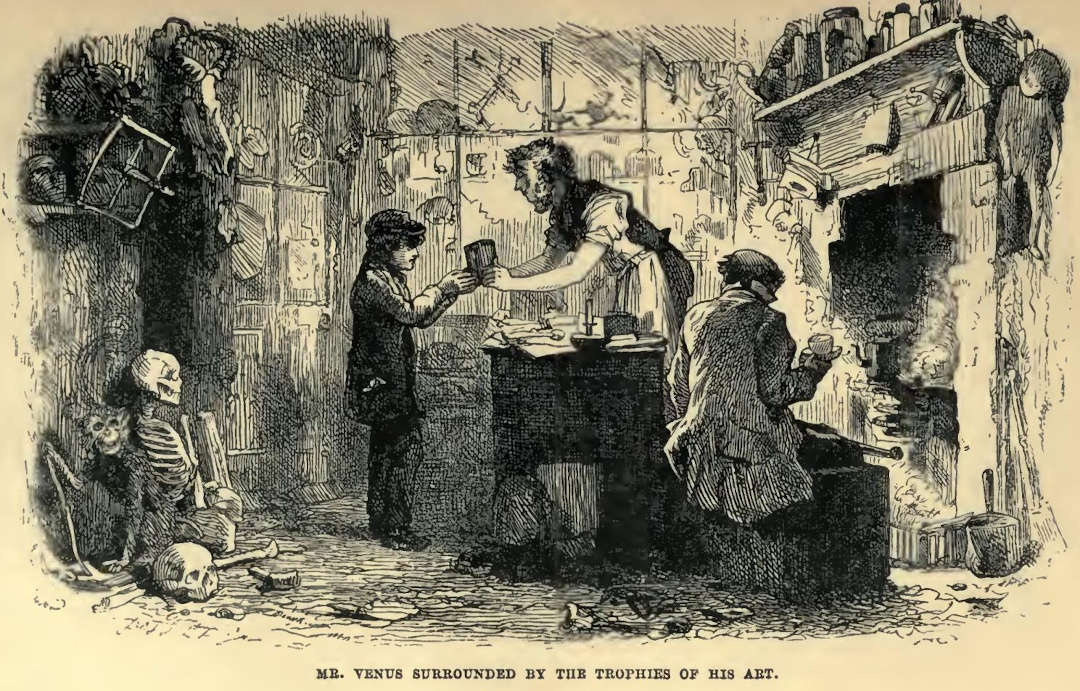
\includegraphics[scale=2.3]{01-07-01}

‘Come for the stuffed canary.’

‘It’s three and ninepence,’ returns Venus; ‘have you got the money?’

The boy produces four shillings. Mr Venus, always in exceedingly low
spirits and making whimpering sounds, peers about for the stuffed
canary. On his taking the candle to assist his search, Mr Wegg observes
that he has a convenient little shelf near his knees, exclusively
appropriated to skeleton hands, which have very much the appearance of
wanting to lay hold of him. From these Mr Venus rescues the canary in a
glass case, and shows it to the boy.

‘There!’ he whimpers. ‘There’s animation! On a twig, making up his mind
to hop! Take care of him; he’s a lovely specimen.--And three is four.’

The boy gathers up his change and has pulled the door open by a leather
strap nailed to it for the purpose, when Venus cries out:

‘Stop him! Come back, you young villain! You’ve got a tooth among them
halfpence.’

‘How was I to know I’d got it? You giv it me. I don’t want none of your
teeth; I’ve got enough of my own.’ So the boy pipes, as he selects it
from his change, and throws it on the counter.

‘Don’t sauce ME, in the wicious pride of your youth,’ Mr Venus retorts
pathetically. ‘Don’t hit ME because you see I’m down. I’m low enough
without that. It dropped into the till, I suppose. They drop into
everything. There was two in the coffee-pot at breakfast time. Molars.’

‘Very well, then,’ argues the boy, ‘what do you call names for?’

To which Mr Venus only replies, shaking his shock of dusty hair, and
winking his weak eyes, ‘Don’t sauce ME, in the wicious pride of your
youth; don’t hit ME, because you see I’m down. You’ve no idea how small
you’d come out, if I had the articulating of you.’

This consideration seems to have its effect on the boy, for he goes out
grumbling.

‘Oh dear me, dear me!’ sighs Mr Venus, heavily, snuffing the candle,
‘the world that appeared so flowery has ceased to blow! You’re casting
your eye round the shop, Mr Wegg. Let me show you a light. My working
bench. My young man’s bench. A Wice. Tools. Bones, warious. Skulls,
warious. Preserved Indian baby. African ditto. Bottled preparations,
warious. Everything within reach of your hand, in good preservation.
The mouldy ones a-top. What’s in those hampers over them again, I don’t
quite remember. Say, human warious. Cats. Articulated English baby.
Dogs. Ducks. Glass eyes, warious. Mummied bird. Dried cuticle, warious.
Oh, dear me! That’s the general panoramic view.’

Having so held and waved the candle as that all these heterogeneous
objects seemed to come forward obediently when they were named, and
then retire again, Mr Venus despondently repeats, ‘Oh dear me, dear
me!’ resumes his seat, and with drooping despondency upon him, falls to
pouring himself out more tea.

‘Where am I?’ asks Mr Wegg.

‘You’re somewhere in the back shop across the yard, sir; and speaking
quite candidly, I wish I’d never bought you of the Hospital Porter.’

‘Now, look here, what did you give for me?’

‘Well,’ replies Venus, blowing his tea: his head and face peering out
of the darkness, over the smoke of it, as if he were modernizing the old
original rise in his family: ‘you were one of a warious lot, and I don’t
know.’

Silas puts his point in the improved form of ‘What will you take for
me?’

‘Well,’ replies Venus, still blowing his tea, ‘I’m not prepared, at a
moment’s notice, to tell you, Mr Wegg.’

‘Come! According to your own account I’m not worth much,’ Wegg reasons
persuasively.

‘Not for miscellaneous working in, I grant you, Mr Wegg; but you might
turn out valuable yet, as a--’ here Mr Venus takes a gulp of tea, so
hot that it makes him choke, and sets his weak eyes watering; ‘as a
Monstrosity, if you’ll excuse me.’

Repressing an indignant look, indicative of anything but a disposition
to excuse him, Silas pursues his point.

‘I think you know me, Mr Venus, and I think you know I never bargain.’

Mr Venus takes gulps of hot tea, shutting his eyes at every gulp, and
opening them again in a spasmodic manner; but does not commit himself to
assent.

‘I have a prospect of getting on in life and elevating myself by my own
independent exertions,’ says Wegg, feelingly, ‘and I shouldn’t like--I
tell you openly I should NOT like--under such circumstances, to be what
I may call dispersed, a part of me here, and a part of me there, but
should wish to collect myself like a genteel person.’

‘It’s a prospect at present, is it, Mr Wegg? Then you haven’t got the
money for a deal about you? Then I’ll tell you what I’ll do with you;
I’ll hold you over. I am a man of my word, and you needn’t be afraid of
my disposing of you. I’ll hold you over. That’s a promise. Oh dear me,
dear me!’

Fain to accept his promise, and wishing to propitiate him, Mr Wegg looks
on as he sighs and pours himself out more tea, and then says, trying to
get a sympathetic tone into his voice:

‘You seem very low, Mr Venus. Is business bad?’

‘Never was so good.’

‘Is your hand out at all?’

‘Never was so well in. Mr Wegg, I’m not only first in the trade, but I’m
THE trade. You may go and buy a skeleton at the West End if you like,
and pay the West End price, but it’ll be my putting together. I’ve as
much to do as I can possibly do, with the assistance of my young man,
and I take a pride and a pleasure in it.’

Mr Venus thus delivers himself, his right hand extended, his smoking
saucer in his left hand, protesting as though he were going to burst
into a flood of tears.

‘That ain’t a state of things to make you low, Mr Venus.’

‘Mr Wegg, I know it ain’t. Mr Wegg, not to name myself as a workman
without an equal, I’ve gone on improving myself in my knowledge of
Anatomy, till both by sight and by name I’m perfect. Mr Wegg, if you was
brought here loose in a bag to be articulated, I’d name your smallest
bones blindfold equally with your largest, as fast as I could pick ‘em
out, and I’d sort ‘em all, and sort your wertebrae, in a manner that
would equally surprise and charm you.’

‘Well,’ remarks Silas (though not quite so readily as last time), ‘THAT
ain’t a state of things to be low about.--Not for YOU to be low about,
leastways.’

‘Mr Wegg, I know it ain’t; Mr Wegg, I know it ain’t. But it’s the heart
that lowers me, it is the heart! Be so good as take and read that card
out loud.’

Silas receives one from his hand, which Venus takes from a wonderful
litter in a drawer, and putting on his spectacles, reads:

‘“Mr Venus,”’

‘Yes. Go on.’

‘“Preserver of Animals and Birds,”’

‘Yes. Go on.’

‘“Articulator of human bones.”’

‘That’s it,’ with a groan. ‘That’s it! Mr Wegg, I’m thirty-two, and a
bachelor. Mr Wegg, I love her. Mr Wegg, she is worthy of being loved by
a Potentate!’ Here Silas is rather alarmed by Mr Venus’s springing to
his feet in the hurry of his spirits, and haggardly confronting him with
his hand on his coat collar; but Mr Venus, begging pardon, sits down
again, saying, with the calmness of despair, ‘She objects to the
business.’

‘Does she know the profits of it?’

‘She knows the profits of it, but she don’t appreciate the art of
it, and she objects to it. “I do not wish,” she writes in her own
handwriting, “to regard myself, nor yet to be regarded, in that boney
light”.’

Mr Venus pours himself out more tea, with a look and in an attitude of
the deepest desolation.

‘And so a man climbs to the top of the tree, Mr Wegg, only to see that
there’s no look-out when he’s up there! I sit here of a night surrounded
by the lovely trophies of my art, and what have they done for me? Ruined
me. Brought me to the pass of being informed that “she does not wish to
regard herself, nor yet to be regarded, in that boney light”!’ Having
repeated the fatal expressions, Mr Venus drinks more tea by gulps, and
offers an explanation of his doing so.

‘It lowers me. When I’m equally lowered all over, lethargy sets in. By
sticking to it till one or two in the morning, I get oblivion. Don’t let
me detain you, Mr Wegg. I’m not company for any one.’

‘It is not on that account,’ says Silas, rising, ‘but because I’ve got
an appointment. It’s time I was at Harmon’s.’

‘Eh?’ said Mr Venus. ‘Harmon’s, up Battle Bridge way?’

Mr Wegg admits that he is bound for that port.

‘You ought to be in a good thing, if you’ve worked yourself in there.
There’s lots of money going, there.’

‘To think,’ says Silas, ‘that you should catch it up so quick, and know
about it. Wonderful!’

‘Not at all, Mr Wegg. The old gentleman wanted to know the nature and
worth of everything that was found in the dust; and many’s the bone, and
feather, and what not, that he’s brought to me.’

‘Really, now!’

‘Yes. (Oh dear me, dear me!) And he’s buried quite in this
neighbourhood, you know. Over yonder.’

Mr Wegg does not know, but he makes as if he did, by responsively
nodding his head. He also follows with his eyes, the toss of Venus’s
head: as if to seek a direction to over yonder.

‘I took an interest in that discovery in the river,’ says Venus.
‘(She hadn’t written her cutting refusal at that time.) I’ve got up
there--never mind, though.’

He had raised the candle at arm’s length towards one of the dark
shelves, and Mr Wegg had turned to look, when he broke off.

‘The old gentleman was well known all round here. There used to be
stories about his having hidden all kinds of property in those dust
mounds. I suppose there was nothing in ‘em. Probably you know, Mr Wegg?’

‘Nothing in ‘em,’ says Wegg, who has never heard a word of this before.

‘Don’t let me detain you. Good night!’

The unfortunate Mr Venus gives him a shake of the hand with a shake of
his own head, and drooping down in his chair, proceeds to pour himself
out more tea. Mr Wegg, looking back over his shoulder as he pulls the
door open by the strap, notices that the movement so shakes the crazy
shop, and so shakes a momentary flare out of the candle, as that the
babies--Hindoo, African, and British--the ‘human warious’, the French
gentleman, the green glass-eyed cats, the dogs, the ducks, and all
the rest of the collection, show for an instant as if paralytically
animated; while even poor little Cock Robin at Mr Venus’s elbow turns
over on his innocent side. Next moment, Mr Wegg is stumping under the
gaslights and through the mud.



